\chapter{Household optimization model}
\label{app:A}
The optimization model discussed in section \ref{submodel} describes how the savings of a household PV-battery configuration can be calculated. To provide some insights into the underlying results of this submodel, an overview of some results will be presented to show the validity of the results the model gives.
\newline \newline \noindent
The main variables of the optimization problem are the net demand $q[t]$, battery charging $ch[t]$, battery discharging $dch[t]$ and battery energy level $e_{BAT}[t]$. The charging and discharging power for a $4kW_p - 5kWh$ battery configuration can be found in figure \ref{figure:charge}.
\newline 
\begin{figure}[h!]
\centering
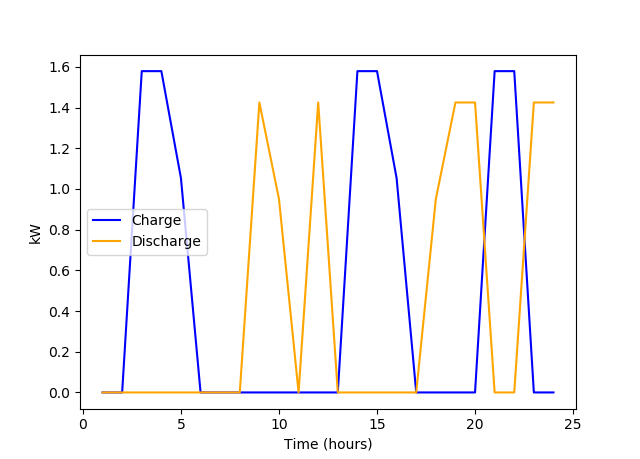
\includegraphics[width=8cm]{(Dis)charge.png}
\caption{Charging and discharging profile of the residential battery}
\label{figure:charge}
\end{figure}
\newline 
The associated energy levels of the battery can be found in figure 
\newline 
\begin{figure}[h!]
\centering
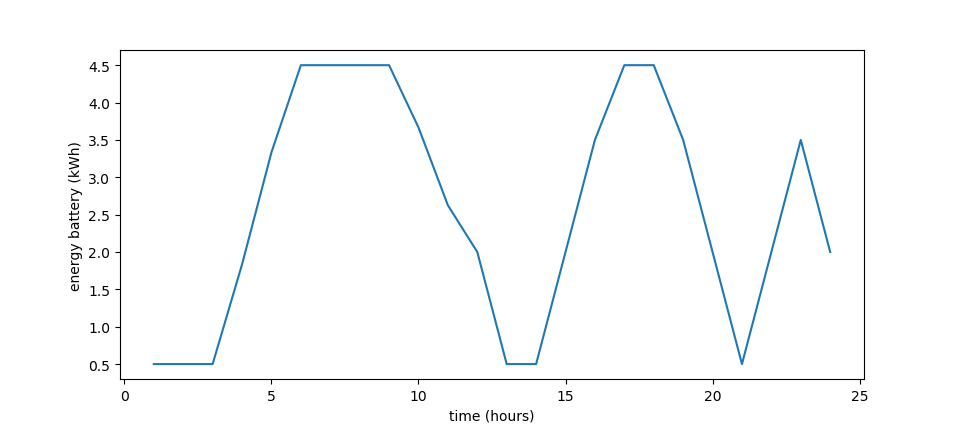
\includegraphics[width=12cm]{energy.png}
\caption{Energy levels battery}
\label{figure:charge}
\end{figure}
\newline
%%% Local Variables: 
%%% mode: latex
%%% TeX-master: "thesis"
%%% End: 
